\section{Synchronisation}
Jeder Thread hat eigener Instruction Pointer, IPs werden unabhängig voneinander bewegt (auch bei Parallelisierung, z.B. wegen Speicherzugriffen)
\subsubsection{Producer-Consumer-Problem}
%\textbf{Producer: }Thread erzeugt Items, \textbf{Consumer: }Thread verarbeitet\\
Threads arbeiten unterschiedlich schnell, Ring-Buffer begrenzt gross

\subssection{Race-Conditions}
\textbf{atomare Instruktion: }1 Instruktion, vom Prozessor unterbrechnungsfrei ausführbar\\
\prgc{++counter} = 3 Instrk., \prgc{inc reg1} = 1 Instrk.\\
\textbf{Race-Condition: }Ergebnisse abhängig von Ausführungsreihenfolge einzelner Instruktionen\\
Nebenläufige Threads im Wettrennen um Hauptspeicher$\rightarrow$Thread-Snych., ausschliessen von Threads notwendig

\subsection{Critical Section}
\textbf{Critical Section: }Code-Bereich der mit anderen Threads geteilt wird\\
\textbf{Anforderungen:} Gegenseitiger Ausschluss (nur 1 Thread in Sect.), 
Fortschritt (Welcher Thread ist nächster?),\\ 
Begrenztes Warten (Thread nur n-mal übergangen, n fix)\\
\textbf{Computer-Arch. $\rightarrow$ keine Garantien:} Instruktionen nicht atomar, Sequenzen werden umgeordnet

\subsection{Mögliche Synchmechanismen mit Hardwaresupport}
\subsubsection{1. Interrupts abschalten}
Alle Interrupts abgeschaltet, wenn in Critical Section\\
\textbf{System mit 1 Prozi:} effektiv, kommt zu keinem Kontext-Wechsel\\
\textbf{Mit mehreren:} Problem: parallele Threads, geht nicht!!\\
\textbf{Generell: } OS kann Thread nicht unterbrechen 

\subsubsection{2. Verwendung von Instruktionen}
%\begin{minted}{C}
%int test_and_set (int *lock){
%int value = *lock;//0 oder 1
%*lock = 1;
%return value;}
%\end{minted}
%Verwendung:
%\begin{minted}{C}
%while (tas (&lock) == 1);//lock nach Aufruf auf 1
%/*critical section*/
%lock = 0;
%\end{minted}
%\begin{minted}{C}
%int compare_and_swap (int *a, int expected, int new_a){
%int value = *a;
%if (value == expected) {*a = new_a;}
%return value; }//alter Wert zurück
%\end{minted}
%Verwendung:
%\begin{minted}{C}
%while (cas (&lock, 0, 1) == 1);//lock nach Aufruf auf 1
%/*critical section*/
%lock = 0;
%\end{minted}
\subsubsection{3. Semaphore}
Zähler z, \prgc{post}: \prgc{z++}, \prgc{wait}: \prgc{z--} falls $z>0$ sonst Thread$\rightarrow$waiting\\
Bsp. für Producer/Consumer, kein Busy-wait mehr
%\begin{multicols*}{2}
%\begin{minted}{C}
%while (1){
%next_produced = produce_next();
%// wait if consumer too slow
%wait ( free );
%buffer [ in ] = next_produced ;
%post ( used );
%in = ( in + 1) % BUFFER_SIZE ;}
%\end{minted}
%\begin{minted}{C}
%while (1){
%// wait if producer too slow
%wait ( used );
%next_consumed = buffer [ out ];
%post ( free );
%out = ( out + 1) % BUFFER_SIZE ;
%consume ( next_consumed );}
%\end{minted}
%\end{multicols*}

\subsubsection{API}
\begin{minted}{C}
sem_t sem; //globale Variable
main{
sem_init(&sem, 0/*nur innerh. Proz. verwendet*/, 4/*init z*/)}
\end{minted}
\begin{minted}{C}
int sem_wait(sem_t *sem);//beide: 0->ok, -1 + errno->Fehler
int sem_post(sem_t *sem);//Fehler-> Semaphore bleibt gleich
\end{minted}
%Wie \prgc{wait} brechen aber ab, wenn Dekrement nicht durchgeführt werden kann:
%\begin{minted}{C}
%int sem_trywait ( sem_t * sem );//sofort
%int sem_timedwait (//nach Timeout
%sem_t * sem , const struct timespec * abs_timeout );
%\end{minted}
Entfernt möglichen zusätzlichen Speicher, den OS mit \prgc{sem} assoziiert hat\\
\prgc{int sem_destroy ( sem_t * sem );}\\
\prgc{sem_getvalue (sem_t * sem, int * out_param);}

\subsubsection{Priority Inversion}
Grund: gemeinsam verwendete Ressource hat niedrigste Prio.\\
Voraussetzungen: 
\begin{itemize}
    \item Ein hoch-priorisierter Thread wartet auf eine Ressource, die von einem niedriger priorisierten Thread gehalten wird
\item Ein Thread mit Priorität zwischen diesen beiden Threads erhält den Prozessor
\end{itemize}
Auswirkung: zugewiesene Prios $\neq$ effektive Prios $\rightarrow$ Inversion

\subsubsection{Priority Inheritance}
\begin{wrapfigure}[6]{l}{0.3\linewidth}
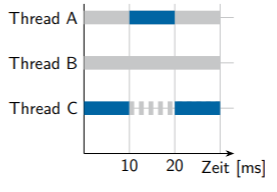
\includegraphics[scale = 0.3]{grafiken/priority_inheritance.PNG} 
\end{wrapfigure}
   
Temporäre Erhöhung der Prio: \\
Thread A hat niedrige Prio und
hält einen Mutex M, Thread B mittel, Thread C hohe und läuft
gerade, Nach 10ms benötigt C M, Prio von A temporär auf
Prio von C/B nicht ausgeführt, A läuft, bis Freigabe von M, Dann läuft wieder C

\subsubsection{4. Mutexe}
\textbf{Acquire/Lock:} Wenn z = 0: \prgc{z = 1}, fahre fort |
wenn z = 1: blockiere Thread bis z = 0
\textbf{Release/Unlock:} setzt z = 0

%\subsubsection{API}
%\begin{minted}{C}
%int pthread_mutex_init (
%pthread_mutex_t * mutex ,
%const pthread_mutexattr_t * attr );//0 falls kein Attr.
%int pthread_mutex_lock ( pthread_mutex_t * mutex );
%int pthread_mutex_trylock ( pthread_mutex_t * mutex );
%int pthread_mutex_unlock ( pthread_mutex_t * mutex );
%int pthread_mutex_destroy ( pthread_mutex_t * mutex );
%\end{minted}



